\subsection{Endliche Automaten und reguläre Sprachen}
Reguläre Sprachen und endliche Automaten gehören zur Automatentheorie, einem Teilbereich der theoretischen Informatik. Zum besseren Verständnis dieser Arbeit wurden folgend einige gängige und wichtige Konzepte der Automatentheorie frei nach dem Standartwerk von Hopcroft, Motwani und Ullman zusammengefasst. \cite{hopcroft}
 
\paragraph{Alphabet}
Ein Alphabet ist eine endliche, nicht leere Menge von Symbolen. Üblicherweise wird ein Alphabet durch das Symbol $\Sigma$ dargestellt.
\paragraph{Zeichenreihen}
Eine Zeichenreihe (auch Wort oder String) ist eine endliche Folge von Symbolen eines bestimmten Alphabetes.
\paragraph{Sprachen}
Eine Menge von Zeichenreihen aus $\Sigma^*$, wobei $\Sigma$ ein bestimmtes Alphabet darstellt, wird als Sprache bezeichnet. Das heisst, eine Sprache ist eine Menge von Zeichenreihen die mit den Zeichen aus einem Alphabet $\Sigma$ gebildet werden können. Bei der Bildung von Wörtern müssen nicht alle Zeichen des gegebenen Alphabets verwendet werden.

Bei der Klasse der regulären Sprachen handelt es sich um die Menge aller Sprachen, welche durch einen endlichen Automaten beschrieben werden können. Alle Sprachen dieser Klasse können auch durch einen regulären Ausdruck dargestellt werden. Das heisst, dass es für jede reguläre Sprache sowohl einen regulären Ausdruck als auch einen endlichen Automaten gibt, der alle Wörter der Sprache akzeptiert.

Ein deterministischer endlicher Automat besteht gemäss Hopcroft, Motwani und Ullman \cite{hopcroft} aus:
\begin{enumerate}
  \item einer endlichen menge von Zuständen die meist durch $Q$ bezeichnet wird.
  \item einer endlichen Menge von Eingabesymbolen (auch Alphabet $\Sigma$).
  \item einer Übergangsfunktion $\delta$ der ein Zustand und ein Eingabesymbol übergeben werden und die einen Zustand zurückgibt.
  \item einem Startzustand welcher Teil der Menge $Q$ sein muss.
  \item einer Menge $F$ akzeptierender Zustände. Die Menge $F$ ist eine Teilmenge von $Q$.
\end{enumerate}

Oft werden endliche Automaten als Quintupel in der Form $A$ = ($Q$, $\Sigma$, $\delta$, $q0$, $F$) dargestellt. 

Zum besseren Verständnis folgend ein Beispiel eines Automaten welcher alle Binärzahlen die durch drei teilbar sind akzeptiert.
\begin{figure}[h]
  \centering
  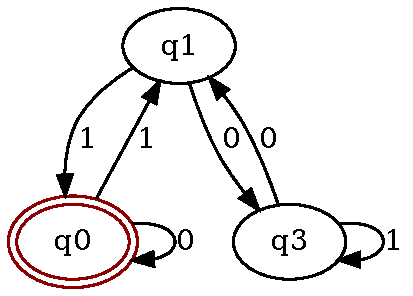
\includegraphics{images/endlicher_automat.pdf}
  \caption[Beispiel: Endlicher Automat]{Beispiel: Endlicher Automat}
  \label{fig:endlicher_automat}
\end{figure}

Die Attribute des Quintupels für diesen Automaten sind:
\begin{enumerate}
	\item $Q$ = \{$q0$, $q1$, $q3$\}
	\item $\Sigma$ = \{$0$, $1$\}
	\item $\delta$
	\item $q0$
	\item $F$ = \{$q0$\}
\end{enumerate}
Wobei man die Übergangsfunktion $\delta$ am einfachsten als Tabelle wie folgt darstellt:
\begin{table}[h]
	\centering
	\begin{tabular}{ c || c | c }
	  \hline
	   & 0 & 1 \\
	  \hline  
	  $\rightarrow$q0* & q0 & q1 \\
	  q1 & q3 & q0 \\
	  q3 & q1 & q3 \\
	  \hline  
	\end{tabular}
	\caption[Übergangstabelle]{Übergangstabelle}
\end{table}

\paragraph{Konventionen}
Ich habe mich bei der Darstellung von Automaten im Rahmen dieser Arbeit auf folgende Konvention festgelegt:
\begin{itemize}
	\item Zustände werden mit einem kleinen q gefolgt von einer Zahl bezeichnet (zB. $q1$)
	\item Zustände müssen nicht durchgängig nummeriert sein
	\item Zustände werden als Ellipsen dargestellt
	\item Zustandsübergänge sind beschriftete Pfeile
	\item der Startzustand erhält einen roten Rand
	\item alle akzeptierenden Zustände sind doppelt umrandet
\end{itemize}